
    %%%%% %%%%% %%%%%
    %               %
    % New row       %
    %               %
    %%%%% %%%%% %%%%%
\begin{columns}[t]
  \begin{column}{0.54\textwidth}
    \begin{block}{\large Copy number does not vary by gene category}
%\small

      \begin{columns}
        \begin{column}{0.5\textwidth}
%\footnotesize
\scriptsize
\vspace{5mm}

Isolates from Mexico typically having two copies of each gene also tended to have two copies of each gene within several annotation categories.
Isolates from South America and US-1 typically had three copies of each gene and also tended to have three copies of each gene within annotation categories.
This indicated that CNV does not prefer particular gene classes.
%          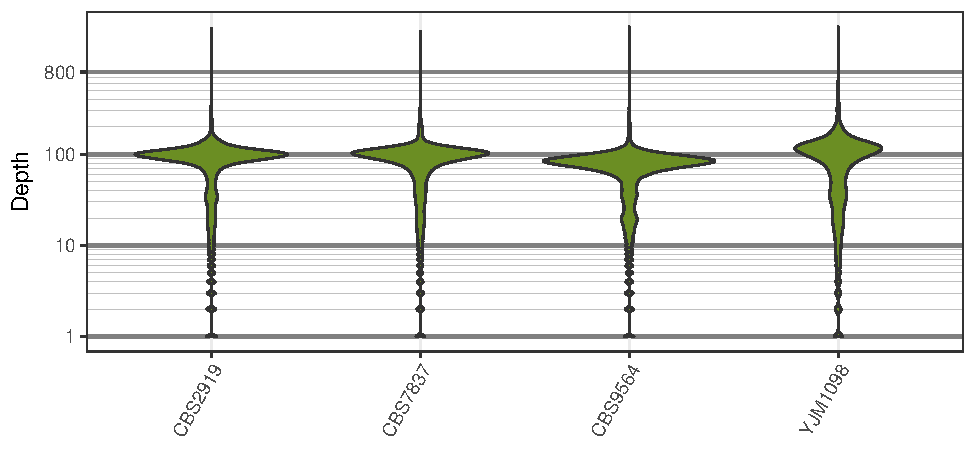
\includegraphics[height=8cm]{./figures/fig2_scer_dp_vplot.pdf}
%          \newline
%          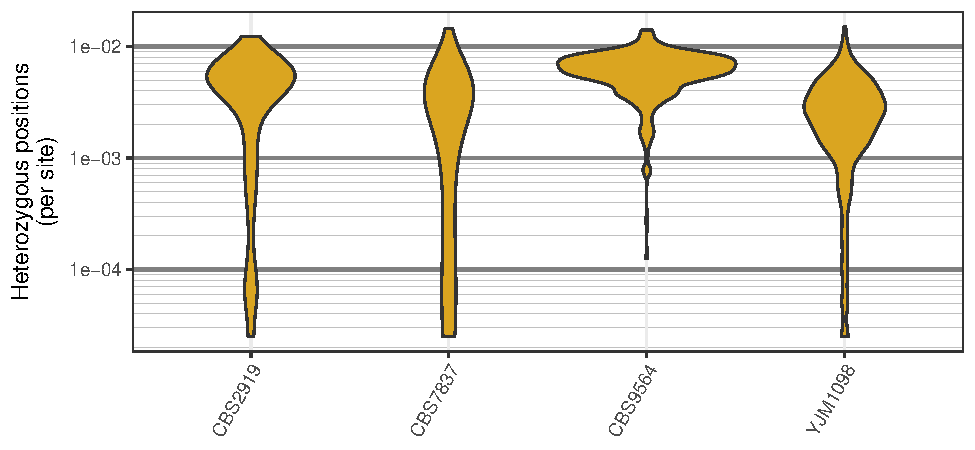
\includegraphics[height=8cm]{./figures/fig3_scer_het_vplot.pdf}
        \end{column}
        \begin{column}{0.45\textwidth}

          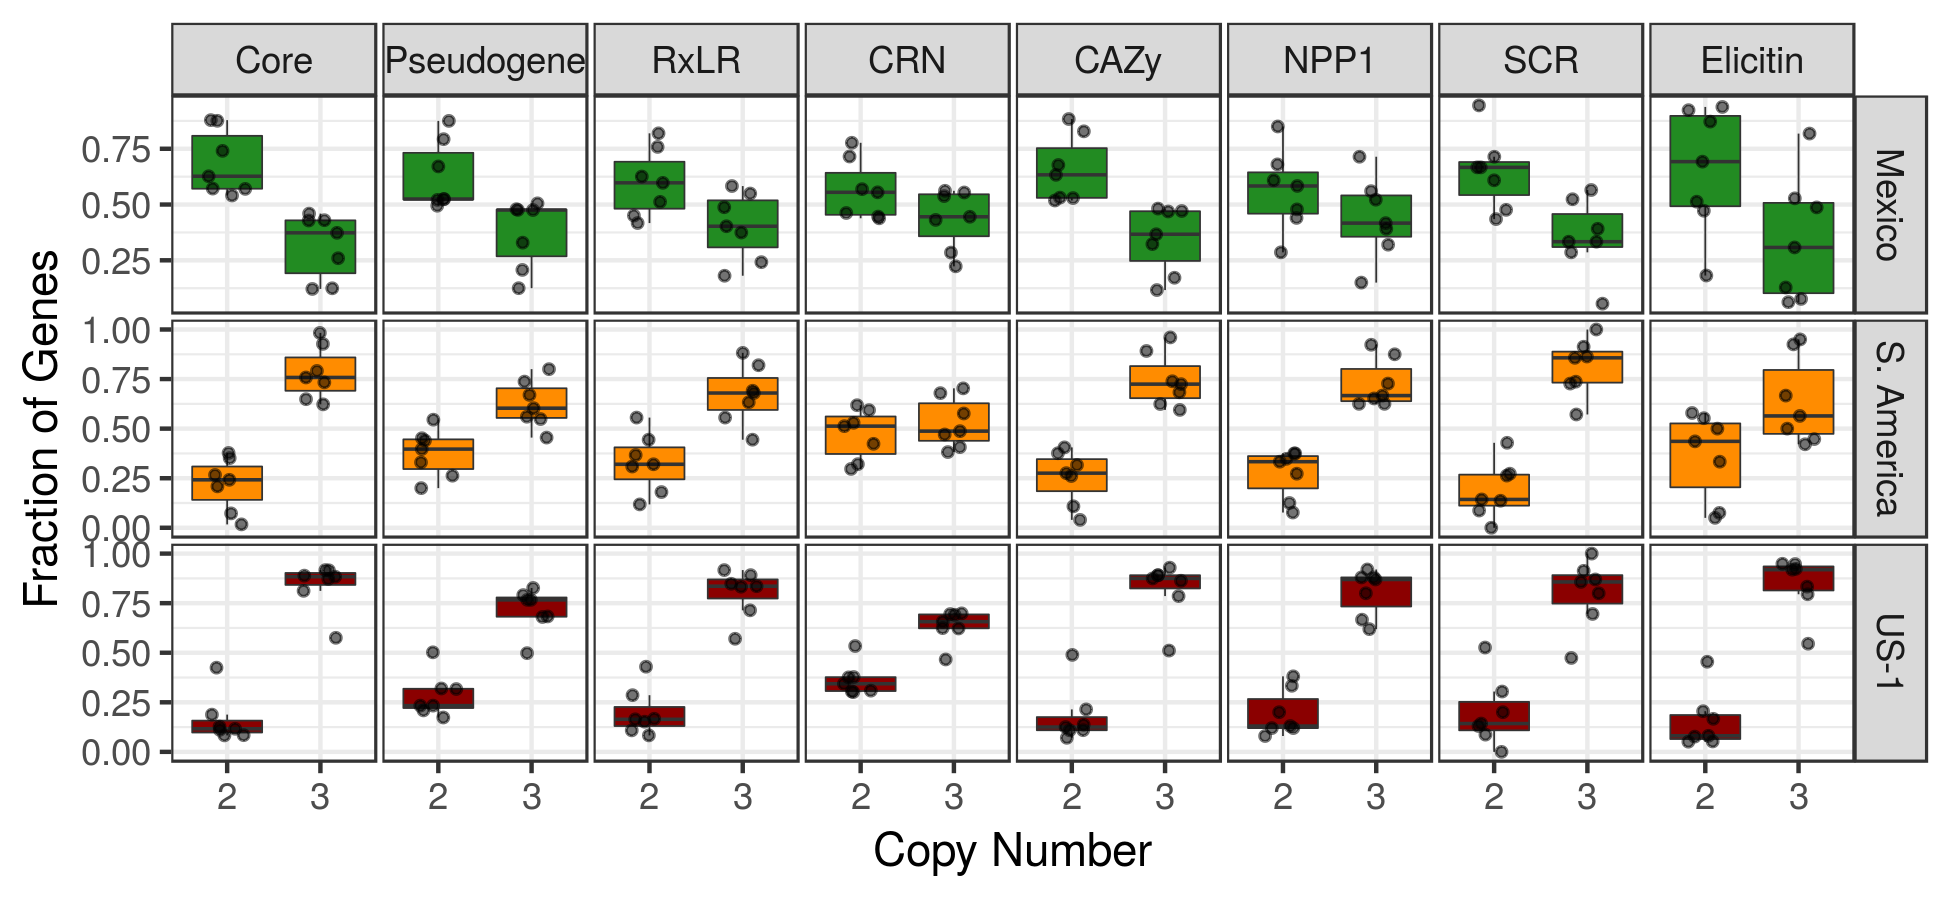
\includegraphics[height=13cm]{./figures/Fig5_gene_cnv.png}

        \end{column}
      \end{columns}

    \end{block}
  \end{column}


  \begin{column}{0.40\textwidth}
    \begin{block}{\large CNV occurs in other species}
      \begin{columns}
        \begin{column}{0.40\textwidth}

          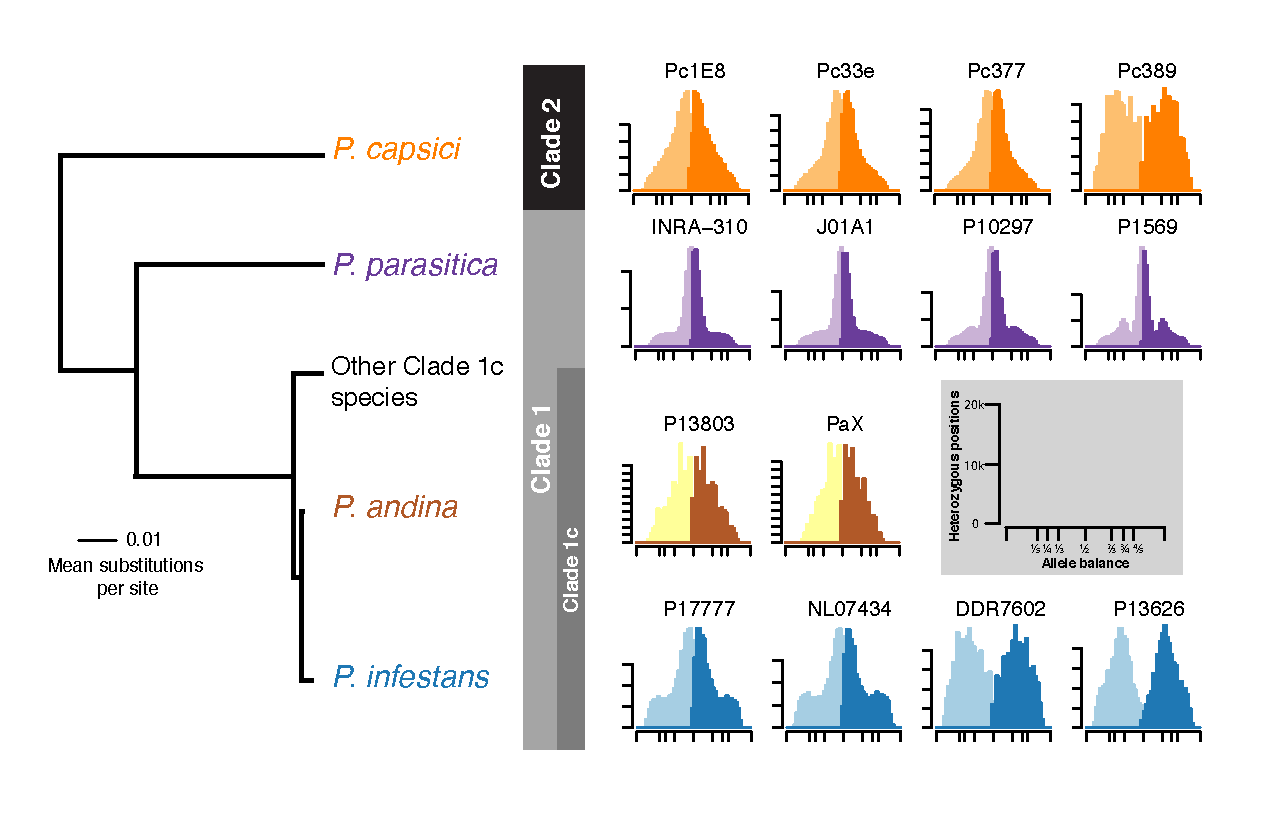
\includegraphics[height=13cm]{./figures/Fig7_ploidy.pdf}

%          \begin{figure}
        \end{column}
        \begin{column}{0.56\textwidth}
%\small
%\footnotesize
\scriptsize
%\tiny
%We used allele balance to explore CNV in other \textit{Phytophthora} genomes that were available at the SRA.
\vspace{5mm}

\textit{P. andina} and \textit{P. parasitica} appeared predominantly diploid.
\textit{P. parasitica} included minor peaks at the expectation for three copies.
Three out of the four \textit{P. capsici} samples appeared predominantly diploid but one appeared triploid.
This indicates that CNV occurs throughout \textit{Phytophthora}.
%          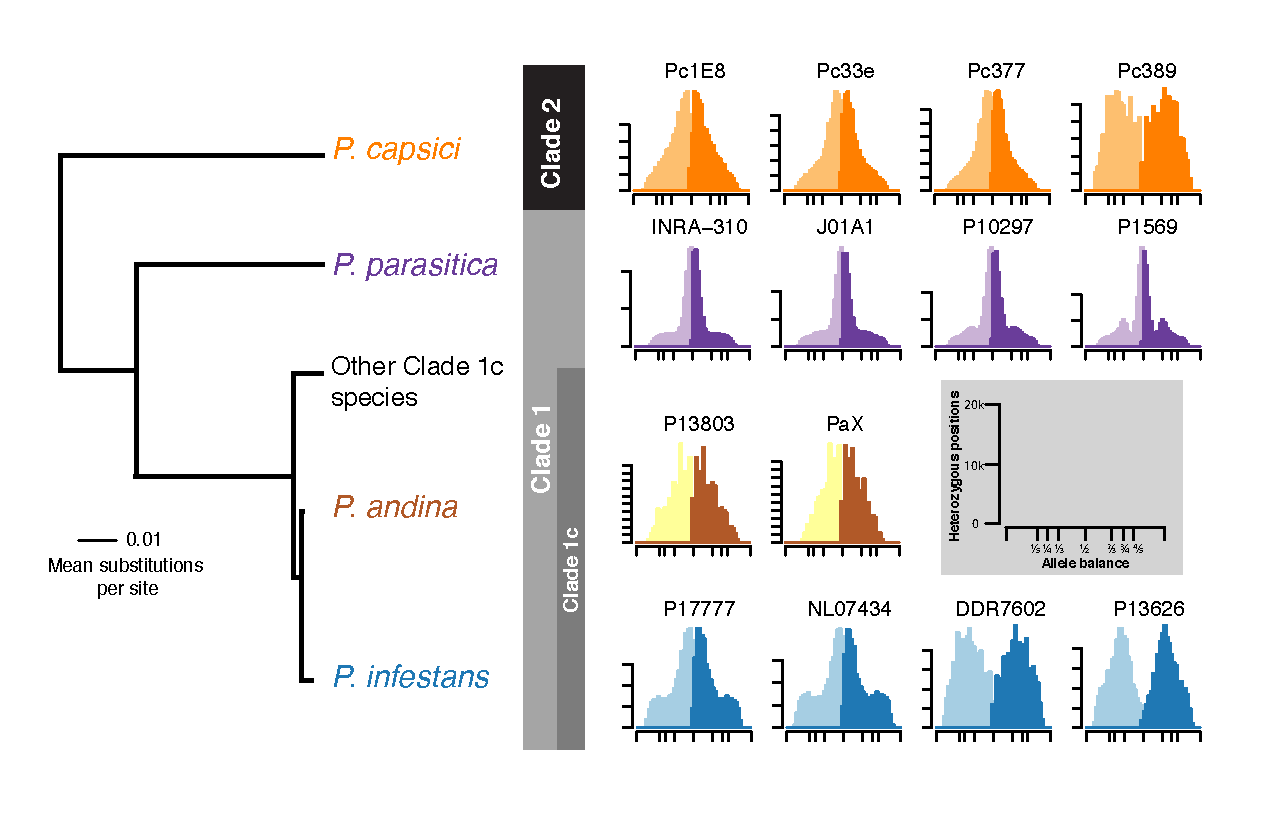
\includegraphics[height=14cm]{./figures/Fig7_ploidy.pdf}
        \end{column}
      \end{columns}
%          \caption{Allele balance is the frequency theat the most abundant and second most abundant allele were sequenced at.}
%          \end{figure}

    \end{block}
  \end{column}


\end{columns}


